\section{W6: Network Protocols, OSI Layers}
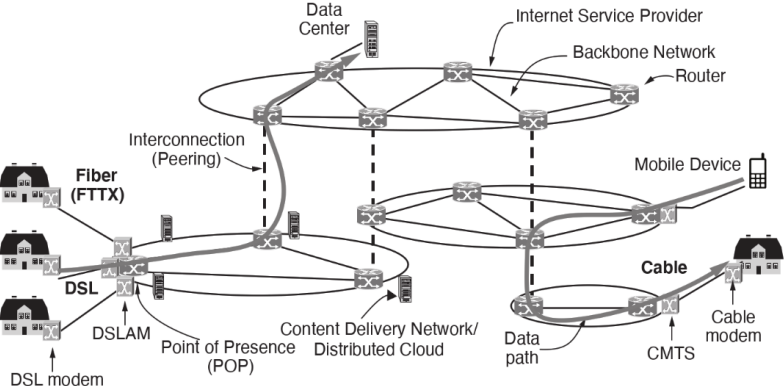
\includegraphics[width=\linewidth]{figs/internet-diagram.png}
\textbf{Two contenders:} TCP/IP and OSI (Open Systems Interconnection). ARPANET used TCP/IP was simpler and won. OSI was too concerned with generality and extensibility.\\
\textbf{OSI model:} is the ideal model that TCP/IP is based on.
\begin{itemize}
    \item A layer should be created where different level of abstraction is needed.
    \item Each layer should perform a well-defined function.
    \item The function of each layer should be chosen with an eye toward defining internationally standardized protocols.
    \item The layer boundaries should be chosen to minimize the information flow across the interfaces.
    \item The number of layers should be large enough that distinct functions need not be thrown together in the same layer out of necessity and small enough that the architecture does not become unwieldy.
\end{itemize}
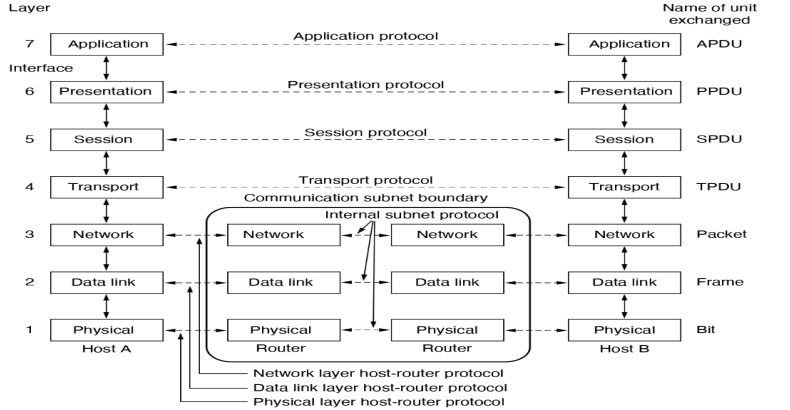
\includegraphics[width=\linewidth]{figs/osi-model.png}
